\documentclass[]{article}
\newcommand{\FileDepth}{../../..}
\usepackage[a4paper, total={15cm,23cm}]{geometry}
\usepackage[T1]{fontenc}
\usepackage{textcomp}%Not strictly necessary, but gives \textmu command for "micro."
\usepackage{fancyhdr}
\usepackage{amsmath}
\usepackage{amssymb}
\usepackage{graphicx}
\usepackage{xcolor}
\usepackage{tikz}
\usetikzlibrary{calc}
\usepackage{cancel}%This is special for Activities 4 and 5.
%opening
\newcommand{\SecType}{R}
\newcommand{\Week}{5}
\title{PH 221 Week \Week}
\author{Benjamin Bauml}
\date{Summer 2024}
\pagestyle{fancy}
\rhead{PH 221}
\chead{Summer 2024}
\lhead{Week \Week}

% For Assignment, leave Purpose as 1. For Worksheet, set to 2. For Student Solution, set to 3. For Teacher Solution, set to 4.
% If you want keep the pieces from being called manually, set DefOnly to 0.
\newcommand{\Purpose}{4}
\newcommand{\DefOnly}{1}

% Version 2024-04-27
% Changes
% 2024-02-21 Added xstring package to enable smooth implementation of new \ModePage command.
% 2024-04-27 Set up to split activities and formatting aspects into separate files. Removed dependence on xcomment. Added an automatic counter to number the activities in a problem set.
\usepackage{tcolorbox}
\usepackage{xstring}
% You will want the following four lines in your document (the last two uncommented):
% For Assignment, leave Purpose as 1. For Worksheet, set to 2. For Student Solution, set to 3. For Teacher Solution, set to 4.
% If you want keep the pieces from being called manually, set DefOnly to 0.
%\newcommand{\Purpose}{4}
%\newcommand{\DefOnly}{1}
\newcommand{\Exclusion}{0}
\newcommand{\PageTurn}{0}
\newcommand{\GrayProb}{0}
\newcommand{\Tipsy}{0}

% Assignment
\if\Purpose1
\renewcommand{\Exclusion}{1}
\fi
% Worksheet
\if\Purpose2
\renewcommand{\Exclusion}{1}
\renewcommand{\PageTurn}{1}
\fi
% Student Solution
\if\Purpose3
\renewcommand{\PageTurn}{1}
\renewcommand{\GrayProb}{1}
\fi
% Teaching Copy
\if\Purpose4
\renewcommand{\PageTurn}{1}
\renewcommand{\GrayProb}{1}
\renewcommand{\Tipsy}{1}
\fi

\def \NewQ {0}
\def \PForce {0}
\newcommand{\MaybePage}[1]{
	\def \PForce {#1}
	\if\PForce1
	\newpage
	\else
	\if\NewQ0
	\gdef \NewQ {\PageTurn}
	\else
	\newpage
	\fi
	\fi
}

\newcommand{\ModePage}[1]{
	\IfSubStr{#1}{\Purpose}{\newpage}{}
}

\newcounter{ActNumber}
\setcounter{ActNumber}{0}

\newcommand{\Problem}[4][0]{%The first argument is optional, and if it is set to 1, the \newpage will be forced. The second argument is the name of the activity, the third is the command the activity is stored as, and the fourth is the actual problem statement.
\newcommand{#3}{
\MaybePage{#1}
\addtocounter{ActNumber}{1}
\section*{\SecType\Week-\theActNumber: #2}
\if\GrayProb1
\begin{tcolorbox}[colback=lightgray,colframe=lightgray,sharp corners,boxsep=1pt,left=0pt,right=0pt,top=0pt,bottom=0pt,after skip=2pt]
\else
\begin{tcolorbox}[colback=white,colframe=white,sharp corners,boxsep=1pt,left=0pt,right=0pt,top=0pt,bottom=0pt,after skip=2pt]
\fi
#4
\end{tcolorbox}\noindent
}
\if\DefOnly0
\else
#3
\fi
}
	
\newcommand{\ProblemSub}[3][0]{%The first argument is optional, and if a string of numbers is entered into it, it will force a \newpage in any \Purpose that shows up in the string. For example, "13" would lead to the newpage being forced in modes 1 and 3. The second is the command the activity is stored as, and the third is the actual problem statement.
\newcommand{#2}{
\ModePage{#1}
\if\GrayProb1
\begin{tcolorbox}[colback=lightgray,colframe=lightgray,sharp corners,boxsep=1pt,left=0pt,right=0pt,top=0pt,bottom=0pt,after skip=2pt]
\else
\begin{tcolorbox}[colback=white,colframe=white,sharp corners,boxsep=1pt,left=0pt,right=0pt,top=0pt,bottom=0pt,after skip=2pt]
\fi
#3
\end{tcolorbox}\noindent
}
\if\DefOnly0
\else
#2
\fi
}
		
\newcommand{\Solution}[2]{%The first argument is the command the solution is stored as, and the second is the actual solution.
\newcommand{#1}{
\if\Exclusion0
#2
\fi
}
\if\DefOnly0
\else
#1
\fi
}
		
\newcommand{\ProblemFig}[2]{%The first argument is the command the figure is stored as, and the second is the actual figure.
\newcommand{#1}{
\begin{figure}[h]
#2
\end{figure}
}
\if\DefOnly0
\else
#1
\fi
}
		
\newcommand{\TeachingTips}[1]{
\if\Tipsy1
\begin{tcolorbox}[colback=lightgray,colframe=black]
#1
\end{tcolorbox}
\fi
}

\newcommand{\FBDaxes}[3]{
	\begin{scope}[shift={(#1)},rotate=#2]
		% x-axis
		\draw[thick,->] (-2,0) -- (2,0);
		\node[anchor=west] at (2,0) {$x$};
		% y-axis
		\draw[thick,->] (0,-2) -- (0,2);
		\node[anchor=west] at (0,2) {$y$};
		\coordinate (#3) at (0,0);
	\end{scope}
}
\newcommand{\FBDvectorMA}[4]{
	\begin{scope}[shift={(#1)}]
		\coordinate (#4tip) at ({#2*cos(#3)},{#2*sin(#3)});
		\draw[ultra thick,blue,->] (#1) -- (#4tip);
	\end{scope}
}
\newcommand{\FBDvectorXY}[3]{
	\begin{scope}[shift={(#1)}]
		\coordinate (#3tip) at (#2);
		\draw[ultra thick,blue,->] (0,0) -- (#3tip);
	\end{scope}
}
\newcommand{\FBDdot}[1]{
	\filldraw[black] (#1) circle (3pt);
}

\begin{document}
\maketitle
\begin{center}
	This material is borrowed/adapted from Chapter 7 of the \textit{Student Workbook} for \textit{Physics for Scientists and Engineers}, and from PH 201 Tutorial 5 for Fall 2020.
\end{center}

\Problem{Interactions and the Third Law}{\InterandThird}{
Draw free-body diagrams and indicate the Newton’s third law pairs for the following situations:
}
\ProblemSub{\InterandThirdA}{
(a) A massless string pulls a box across the floor. Friction is not negligible.
}
\Solution{\InterandThirdASol}{
\begin{figure}[h]
	\centering
	\begin{tikzpicture}
		\FBDaxes{0,0}{0}{axes}
		%This is just to test the FBDbox command.
		%\FBDbox{2,2}{0}{box}{$m$}
		%\draw (boxbr) -- (2,0) -- (boxtr) -- (0,2) -- (boxtl) -- (-2,0) -- (boxbl) -- (0,-2) -- cycle;
		%\draw (boxrbq) -- (2,0) -- (boxrtq) -- (boxtrq) -- (0,2) -- (boxtlq) -- (boxltq) -- (-2,0) -- (boxlbq) -- (boxblq) -- (0,-2) -- (boxbrq) -- cycle;
		%\draw (2,0) -- (boxrcent);
		%\draw (-2,0) -- (boxlcent);
		%\draw (0,2) -- (boxtcent);
		%\draw (0,-2) -- (boxbcent);
		\FBDbox[0.8]{axes}{0}{box}{}
		\FBDvectorXY{boxrcent}{0.7,0}{FT}
		\node[anchor=south] at (FTtip) {$\vec{F}^{T}_{BS}$};
		\FBDvectorXY{boxlcent}{-0.7,0}{FK}
		\node[anchor=south] at (FKtip) {$\vec{F}^{kf}_{BF}$};
		\FBDvectorXY{boxtcent}{0,1}{FN}
		\node[anchor=west] at (FNtip) {$\vec{F}^{N}_{BF}$};
		\FBDvectorXY{boxbcent}{0,-1}{FG}
		\node[anchor=west] at (FGtip) {$\vec{F}^{g}_{BE}$};
	\end{tikzpicture}
\end{figure}

There are no 3rd law pairs in my above representation, as I only drew one free-body diagram. Technically, each of these forces is part of a 3rd law pair ($\vec{F}^{N}_{BF}$ with $\vec{F}^{N}_{FB}$, $\vec{F}^{kf}_{BF}$ with $\vec{F}^{kf}_{FB}$, $\vec{F}^{T}_{BS}$ with $\vec{F}^{T}_{SB}$, and $\vec{F}^{g}_{BE}$ with $\vec{F}^{g}_{EB}$), but since I didn't draw free-body diagrams for the floor, the string, or the Earth, the other vector of each pair is not present.

We know that the normal and gravitational forces are balanced on this box, though we don't know if the force of tension is balanced against the force of kinetic friction. I drew them equal for simplicity, but if we had more information about the box's acceleration, we might want to redraw them with different lengths.
}
\ProblemSub[34]{\InterandThirdB}{
(b) The bottom block is pulled by a massless string. Friction is not negligible. Treat the two blocks as separate objects.
}
\ProblemFig{\InterandThirdBFig}{
\centering
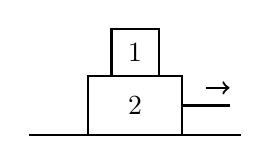
\begin{tikzpicture}
	\begin{scope}[scale=1.5]
	\draw[thick] (0,0) rectangle (0.8,0.5);
	\node at (0.4,0.25) {2};
	\draw[thick] (0.2,0.5) rectangle (0.6,0.9);
	\node at (0.4,0.7) {1};
	\draw[thick] (0.8,0.25) -- (1.2,0.25);
	\draw[thick] (-0.5,0) -- (1.3,0);
	\draw[thick,->] (1,0.4) -- (1.2,0.4);
	\end{scope}
\end{tikzpicture}
}
\Solution{\InterandThirdBSol}{

If the blocks are speeding up, then I would draw the following diagrams:

\begin{figure}[h]
	\centering
	\begin{tikzpicture}
		\FBDaxes{-3,0}{0}{taxes}
		\FBDbox[0.8]{taxes}{0}{tbox}{1}
		\FBDvectorXY{tboxrcent}{0.7,0}{FS12}
		\node[anchor=south] at (FS12tip) {$\vec{F}^{sf}_{12}$};
		\FBDvectorXY{tboxtcent}{0,1}{FN12}
		\node[anchor=west] at (FN12tip) {$\vec{F}^{N}_{12}$};
		\FBDvectorXY{tboxbcent}{0,-1}{FG1}
		\node[anchor=west] at (FG1tip) {$\vec{F}^{g}_{1E}$};
		\FBDaxes[3]{3,0}{0}{baxes}
		\FBDbox{baxes}{0}{bbox}{2}
		\FBDvectorXY{bboxltq}{-0.7,0}{FS21}
		\node[anchor=south] at (FS21tip) {$\vec{F}^{sf}_{21}$};
		\FBDvectorXY{bboxblq}{0,-1}{FN21}
		\node[anchor=east] at (FN21tip) {$\vec{F}^{N}_{21}$};
		\FBDvectorXY{bboxlbq}{-1.1,0}{FK}
		\node[anchor=north] at (FKtip) {$\vec{F}^{kf}_{2G}$};
		\FBDvectorXY{bboxrcent}{2,0}{FT}
		\node[anchor=north] at (FTtip) {$\vec{F}^{T}_{2S}$};
		\FBDvectorXY{bboxbcent}{0,-1.3}{FG2}
		\node[anchor=west] at (FG2tip) {$\vec{F}^{g}_{2E}$};
		\FBDvectorXY{bboxtcent}{0,2.3}{FN2}
		\node[anchor=west] at (FN2tip) {$\vec{F}^{N}_{2G}$};
	\end{tikzpicture}
\end{figure}

We can see that the static friction from block 2 pulls block 1 to the right, and therefore the static friction from block 1 pulls block 2 in the opposite direction, working against its motion.

On the other hand, if the blocks are slowing down, I would instead draw the following diagrams:

\begin{figure}[h]
	\centering
	\begin{tikzpicture}
		\FBDaxes{-3,0}{0}{taxes}
		\FBDbox[0.8]{taxes}{0}{tbox}{1}
		\FBDvectorXY{tboxlcent}{-0.7,0}{FS12}
		\node[anchor=south] at (FS12tip) {$\vec{F}^{sf}_{12}$};
		\FBDvectorXY{tboxtcent}{0,1}{FN12}
		\node[anchor=west] at (FN12tip) {$\vec{F}^{N}_{12}$};
		\FBDvectorXY{tboxbcent}{0,-1}{FG1}
		\node[anchor=west] at (FG1tip) {$\vec{F}^{g}_{1E}$};
		\FBDaxes[3]{3,0}{0}{baxes}
		\FBDbox{baxes}{0}{bbox}{2}
		\FBDvectorXY{bboxrtq}{0.7,0}{FS21}
		\node[anchor=south] at (FS21tip) {$\vec{F}^{sf}_{21}$};
		\FBDvectorXY{bboxblq}{0,-1}{FN21}
		\node[anchor=east] at (FN21tip) {$\vec{F}^{N}_{21}$};
		\FBDvectorXY{bboxlbq}{-1.1,0}{FK}
		\node[anchor=north] at (FKtip) {$\vec{F}^{kf}_{2G}$};
		\FBDvectorXY{bboxrcent}{0.2,0}{FT}
		\node[anchor=north west] at (FTtip) {$\vec{F}^{T}_{2S}$};
		\FBDvectorXY{bboxbcent}{0,-1.3}{FG2}
		\node[anchor=west] at (FG2tip) {$\vec{F}^{g}_{2E}$};
		\FBDvectorXY{bboxtcent}{0,2.3}{FN2}
		\node[anchor=west] at (FN2tip) {$\vec{F}^{N}_{2G}$};
	\end{tikzpicture}
\end{figure}

We can see here that the static friction on 1 by 2 must act to slow down block 1, but the static friction on 2 by 1 points in the same direction as the motion---in a sense, the bottom block can feel the top block trying to keep going forward at its original speed.

The third law pairs here are the static frictions, $\vec{F}^{sf}_{12}$ and $\vec{F}^{sf}_{21}$, and the normal forces between the blocks, $\vec{F}^{N}_{12}$ and $\vec{F}^{N}_{21}$.
}
\ProblemSub[34]{\InterandThirdC}{
(c) A skateboarder is pushing on the ground to speed up. Treat the person and the skateboard as separate objects.
}
\Solution{\InterandThirdCSol}{The person has one foot on the board (so there will be a normal and a frictional force from that) and one foot on the ground (so there will be a normal and a frictional force from that). With the long range force of gravity, that makes five forces total on the person.

The board is touching the person (so there will be a normal and a frictional force from that) and the ground (so there will be a normal and a frictional force from that). With the long range force of gravity, that makes five forces total on the skateboard as well.

\begin{figure}[h]
	\centering
	\begin{tikzpicture}
		\FBDaxes{-2.5,0}{0}{paxes}
		\FBDbox[0.6]{paxes}{0}{pbox}{P}
		\FBDvectorXY{pboxtrq}{0,1}{FNPS}
		\node[anchor=west] at (FNPStip) {$\vec{F}^{N}_{PS}$};
		\FBDvectorXY{pboxtlq}{0,0.8}{FNPG}
		\node[anchor=east] at (FNPGtip) {$\vec{F}^{N}_{PG}$};
		\FBDvectorXY{pboxbcent}{0,-1.8}{FGP}
		\node[anchor=west] at (FGPtip) {$\vec{F}^{g}_{PE}$};
		\FBDvectorXY{pboxlcent}{-0.6,0}{FSPS}
		\node[anchor=north] at (FSPStip) {$\vec{F}^{sf}_{PS}$};
		\FBDvectorXY{pboxrcent}{1,0}{FSPG}
		\node[anchor=north] at (FSPGtip) {$\vec{F}^{sf}_{PG}$};
		\FBDaxes{2.5,0}{0}{saxes}
		\FBDbox[0.6]{saxes}{0}{sbox}{S}
		\FBDvectorXY{sboxbrq}{0,-1}{FNSP}
		\node[anchor=west] at (FNSPtip) {$\vec{F}^{N}_{SP}$};
		\FBDvectorXY{sboxtcent}{0,1.6}{FNSG}
		\node[anchor=east] at (FNSGtip) {$\vec{F}^{N}_{SG}$};
		\FBDvectorXY{sboxblq}{0,-0.6}{FGS}
		\node[anchor=east] at (FGStip) {$\vec{F}^{g}_{SE}$};
		\FBDvectorXY{sboxrcent}{0.6,0}{FSSP}
		\node[anchor=north] at (FSSPtip) {$\vec{F}^{sf}_{SP}$};
		\FBDvectorXY{sboxlcent}{-0.4,0}{FRSG}
		\node[anchor=south] at (FRSGtip) {$\vec{F}^{rf}_{SG}$};
	\end{tikzpicture}
\end{figure}

In drawing these, I assumed that the person and skateboard are speeding up to the right. As such, the person is pushing backward (to the left) against the ground with their foot, which means the static friction from the ground must point right to keep the foot from slipping backward. As such, this static friction is what propels the person forward (to the right). Similarly, the static friction on the board by the person's other foot also propels the skateboard forward with the skateboarder. Conversely, the static friction on the skateboarder by the skateboard points to the left; the person feels dragged backward a bit as the skateboard's inertia resists being dragged along with them.

The third law pairs are the forces of static friction between the person and the skateboard ($\vec{F}^{sf}_{PS}$ and $\vec{F}^{sf}_{SP}$) and the normal forces between the person and the skateboard ($\vec{F}^{N}_{PS}$ and $\vec{F}^{N}_{SP}$).

As a side note, you may notice that I labeled the friction between the skateboard and the ground as $\vec{F}^{rf}_{SG}$. We don't teach this in the course, but $rf$ is meant to stand for a third friction model: \textit{rolling friction}. The important thing is, we cannot call this friction between the board and the ground kinetic. Kinetic friction is only for things sliding against each other, and here, the wheels do not slip against the ground. Since the wheels are not slipping, you could think of there being a force of static friction that keeps the wheels from slipping (they would be sliding to the right if there were no friction, so this static friction would still point left in this case, where the wheels are not propelling the skateboard---unlike an FBD for a car). However, rolling friction is more accurate, as it captures the additional interactions inherent in a surface sinking into and lifting off from another surface as it rolls across.
}
\Problem{Two Blocks on a Frictionless Half-Ramp}{\TBFricHRamp}{
Consider the situation depicted below. Friction is negligible for the blocks and surface, and we will assume the strings and pulley are ideal (massless, frictionless, etc.).
}
\ProblemFig{\TBFricHRampFig}{
\centering
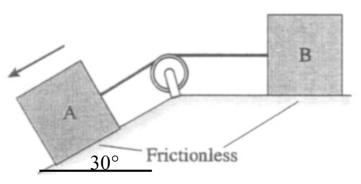
\includegraphics[scale=1.2]{\FileDepth/Activities/Two_Blocks_on_a_Frictionless_Half-Ramp/Blocks_on_a_Half-Tilt_Frictionless}
}
\ProblemSub{\TBFricHRampA}{
(a) Draw a free-body diagram for each block.
}
\Solution{\TBFricHRampASol}{I will indicate the half-ramp with the subscript $R$ and the string with the subscript $S$.

\begin{figure}[h]
	\centering
	\begin{tikzpicture}
		\FBDaxes{-2.5,0}{30}{Aaxes}
		\FBDbox[0.6]{Aaxes}{30}{Abox}{A}
		\FBDvectorXY{Aboxblq}{0,-1.5}{FGA}
		\node[anchor=east] at (FGAtip) {$\vec{F}^{g}_{AE}$};
		\FBDvectorMA{Aboxrcent}{0.75}{30}{FTA}
		\node[anchor=south] at (FTAtip) {$\vec{F}^{T}_{AS}$};
		\FBDvectorMA{Aboxtcent}{1.3}{120}{FNA}
		\node[anchor=east] at (FNAtip) {$\vec{F}^{N}_{AR}$};
		\draw[thick] (-2.5,-0.7) arc (270:300:0.7);
		\node[anchor=north] at (-2.3,-0.7) {$\theta$};
		\begin{scope}[shift={(-2.5,0)}]
			\draw[thick,dashed] ({-2*cos(30)},-1) -- ({-2*cos(30)+1},-1);
			\draw[thick] ({-2*cos(30)+0.7},-1) arc (0:30:0.7);
			\node[anchor=south west] at ({-2*cos(30)+0.7},-1) {$\theta$};
		\end{scope}
		\FBDaxes{2.5,0}{0}{Baxes}
		\FBDbox[0.6]{Baxes}{0}{Bbox}{B}
		\FBDvectorXY{Bboxbcent}{0,-1.5}{FGB}
		\node[anchor=west] at (FGBtip) {$\vec{F}^{g}_{BE}$};
		\FBDvectorXY{Bboxtcent}{0,1.5}{FNB}
		\node[anchor=west] at (FNBtip) {$\vec{F}^{N}_{BR}$};
		\FBDvectorXY{Bboxlcent}{-0.75,0}{FTB}
		\node[anchor=south] at (FTBtip) {$\vec{F}^{T}_{BS}$};
	\end{tikzpicture}
\end{figure}
}
\TeachingTips{
This is one problem where it is imperative \underline{not} to use $G$ for ``ground'' to indicate the surface beneath the blocks. If you do, the force on block A by the ground will have a very unfortunate symbol: $\vec{F}_{AG}$. It may be rather uncomfortable to accidentally write something that looks like a slur in front of your students.
}
\ProblemSub{\TBFricHRampB}{
(b) Indicate the Newton’s third law pairs.
}
\Solution{\TBFricHRampBSol}{There are no third law pairs. $\vec{F}^{T}_{AS}$ and $\vec{F}^{T}_{BS}$ are equal in magnitude, but they are not opposite in direction, and they are not directly between boxes A and B, instead going through the string and pulley between them.

However, since these two forces are equal in magnitude (due to the ideality of the pulley and the string), I will simplify my notation by giving their magnitudes a single symbol: $F^{T} = F^{T}_{AS} = F^{T}_{BS}$.
}
\ProblemSub{\TBFricHRampC}{
(c) Find the normal force on each block.
}
\Solution{\TBFricHRampCSol}{In order to do this, I will write out Newton's second law in the $y$-direction for both blocks. Neither is accelerating perpendicular to the surface, so the net force in this direction is zero.
\begin{align*}
F^{net}_{A,y} & = F^{N}_{AR,y}+F^{g}_{AE,y} & F^{net}_{B,y} & = F^{N}_{BR,y}+F^{g}_{BE,y} \\
0 & = F^{N}_{AR}-m_{A}g\cos\theta & 0 & = F^{N}_{BR}-m_{B}g \\
F^{N}_{AR} & = m_{A}g\cos\theta & F^{N}_{BR} & = m_{B}g
\end{align*}
}
\ProblemSub{\TBFricHRampD}{
(d) Find the acceleration of the two blocks.
}
\Solution{\TBFricHRampDSol}{Both blocks accelerate in the $x$-direction, and since they are attached, they must have the same magnitude of acceleration. Also, since their coordinate systems agree on which direction along the surface is $+x$, the accelerations will also share the same sign. As such, I will use a single symbol for both accelerations: $a = a_{A,x} = a_{B,x}$.
\begin{align*}
	F^{net}_{A,x} & = F^{T}_{AS,x}+F^{g}_{AE,x} & F^{net}_{B,x} & = F^{T}_{BS,x} \\
	m_{A}a_{A,x} & = F^{T}-m_{A}g\sin\theta & m_{B}a_{B,x} & = -F^{T} \\
	m_{A}a & = F^{T}-m_{A}g\sin\theta & m_{B}a & = -F^{T}
\end{align*}
Adding these two equations together gives us
\begin{align*}
	(m_{A}+m_{B})a & = F^{T}-m_{A}g\sin\theta + (-F^{T}) = -m_{A}g\sin\theta \\
	a & = -\frac{m_{A}}{m_{A}+m_{B}}g\sin\theta
\end{align*}
The negative sign lets us know that these blocks will accelerate to the left.

In the special case where $m_{B} \ll m_{A}$, the fraction $\frac{m_{A}}{m_{A}+m_{B}}$ approaches 1, and we get $a = g\sin\theta$, which is the acceleration we expect from an object freely sliding down a ramp (which we expect to be the limiting case when there is no additional mass attached to A). Conversely, if $m_{B} \gg m_{A}$, then $\frac{m_{A}}{m_{A}+m_{B}} \approx \frac{m_{A}}{m_{B}} \approx 0$, and the blocks don't move. This we also expect, as a massive enough block B should not allow block A to move it, thus preventing any sliding.
}
\ProblemSub{\TBFricHRampE}{
(e) Find the tension in the string.
}
\Solution{\TBFricHRampESol}{We already know from part (d) that $F^{T} = -m_{B}a$, so we can substitute our answer for the acceleration into this to obtain
\[
F^{T} = \frac{m_{A}m_{B}}{m_{A}+m_{B}}g\sin\theta.
\]
If we wanted to do more algebra, we could also start with both equations from (d) and solve them for $F^{T}$ instead of for $a$:
\begin{align*}
	m_{A}a & = F^{T}-m_{A}g\sin\theta & m_{B}a & = -F^{T} \\
	m_{A}m_{B}a & = m_{B}F^{T}-m_{A}m_{B}g\sin\theta & m_{A}m_{B}a & = -m_{A}F^{T}
\end{align*}
Subtracting the right hand equation from the left hand equation gives us
\begin{align*}
	m_{A}m_{B}a - m_{A}m_{B}a & = m_{B}F^{T}-m_{A}m_{B}g\sin\theta - (-m_{A}F^{T}) \\
	0 & = (m_{A}+m_{B})F^{T} - m_{A}m_{B}g\sin\theta \\
	F^{T} & = \frac{m_{A}m_{B}}{m_{A}+m_{B}}g\sin\theta.
\end{align*}
Our answer is positive (for all sensible angles from 0$^{\circ}$ to 90$^{\circ}$), which should be the case for a magnitude of a vector. Sometimes, when we do force analysis and get a negative number, it just tells us that the direction we assumed for a force is backward from what it actually is, but in this case, getting a negative magnitude would tell us that something was wrong. After all, tension cannot push.

For $m_{A} \gg m_{B}$, we obtain $F^{T} \approx \frac{m_{A}m_{B}}{m_{A}}g\sin\theta = m_{B}g\sin\theta$. In this situation (as I mentioned in part (d)), block A is accelerating at $g\sin\theta$ down the ramp, so the force on block B needs to be just perfect to get it accelerating at $g\sin\theta$ to keep up.

Conversely, for $m_{B} \gg m_{A}$, we obtain $F^{T} \approx \frac{m_{A}m_{B}}{m_{B}}g\sin\theta = m_{A}g\sin\theta$. In this situation, both blocks are stationary (B is too massive to move), so the tension needs to be strong enough to counteract the $x$-component of the force of gravity on A and hold it in place.
}
\end{document}